\documentclass{article}
\usepackage{epsfig}
\usepackage{graphicx}
\usepackage[top=0.50in, bottom=0.50in, left=0.65in, right=0.75in]{geometry}
%\usepackage[a4paper, total={6in, 10in}]{geometry}
\usepackage[table]{xcolor}
\usepackage{tikz}
\usepackage{algorithm}
\usepackage{mathtools}
\usepackage{amsmath,amssymb}
\usepackage[]{algpseudocode}
\usepackage{enumitem}
\title{CS345 Theoretical Assignment 3 \\ }
\author{\vspace{2mm} \large Ayush Agarwal, 13180 \\ M.Arunothia, 13378}
\date{}
\begin{document}
\maketitle
\tableofcontents
\newpage
\section{Mobile Network}
\subsection{Overview}
We take Dynamic Programming approach to solve this problem. The overview of our solution can be described using the following cost matrix. $cost[i][j]$ stores the cost structure (see pseudo code) for corresponding paths that lead to least cost($P_i,..P_j$). To estimate the column green, we will have everything in blue already estimated. We will traverse this column bottom up. To estimate the red box, we will need those boxes shown by the red arrow.    
\begin{center}
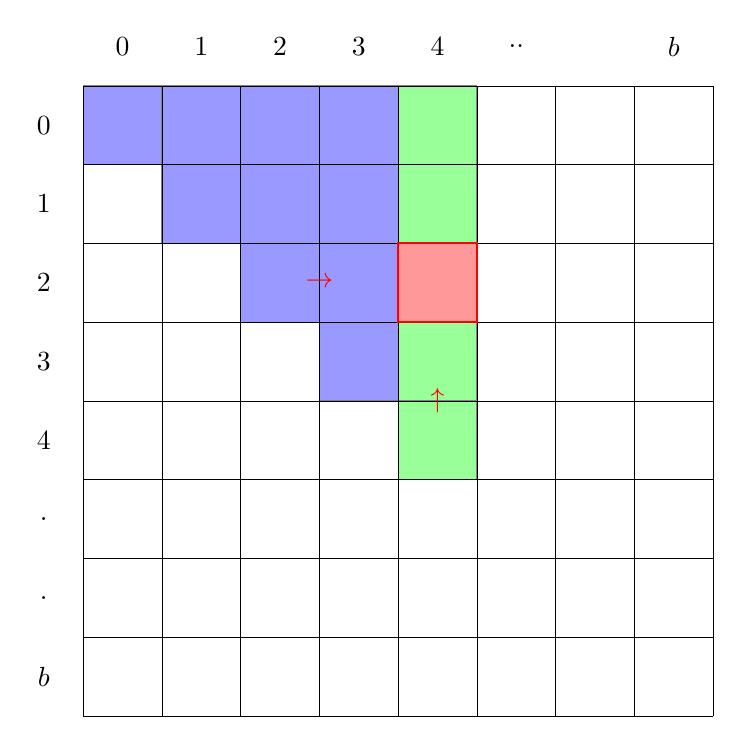
\begin{tikzpicture}
\node at (-1.5,6.5) {$0$};
\node at (-0.5,6.5) {$1$};
\node at (0.5,6.5) {$2$};
\node at (1.5,6.5) {$3$};
\node at (2.5,6.5) {$4$};
\node at (3.5,6.5) {$..$};
\node at (5.5,6.5) {$b$};
\node at (-2.5,5.5) {$0$};
\node at (-2.5,4.5) {$1$};
\node at (-2.5,3.5) {$2$};
\node at (-2.5,2.5) {$3$};
\node at (-2.5,1.5) {$4$};
\node at (-2.5,0.5) {$.$};
\node at (-2.5,-0.5) {$.$};
\node at (-2.5,-1.5) {$b$};
\filldraw[fill=blue!40!white, draw=gray] (-2,5) rectangle (-1,6);
\filldraw[fill=blue!40!white, draw=gray] (-1,5) rectangle (0,6);
\filldraw[fill=blue!40!white, draw=gray] (-1,4) rectangle (0,5);
\filldraw[fill=blue!40!white, draw=gray] (0,5) rectangle (1,6);
\filldraw[fill=blue!40!white, draw=gray] (0,4) rectangle (1,5);
\filldraw[fill=blue!40!white, draw=gray] (0,3) rectangle (1,4);
\filldraw[fill=blue!40!white, draw=gray] (1,5) rectangle (2,6);
\filldraw[fill=blue!40!white, draw=gray] (1,4) rectangle (2,5);
\filldraw[fill=blue!40!white, draw=gray] (1,3) rectangle (2,4);
\filldraw[fill=blue!40!white, draw=gray] (1,2) rectangle (2,3);
\filldraw[fill=green!40!white, draw=gray] (2,5) rectangle (3,6);
\filldraw[fill=green!40!white, draw=gray] (2,4) rectangle (3,5);
\filldraw[fill=green!40!white, draw=gray] (2,2) rectangle (3,3);
\filldraw[fill=green!40!white, draw=gray] (2,1) rectangle (3,2);
\draw[step=1cm,black,very thin] (-2,-2) grid (6,6);
\node[red] at (1,3.5) {$\rightarrow$};
\node[red] at (2.5,2) {$\uparrow$};
\filldraw[fill=red!40!white, draw=red, thick] (2,3) rectangle (3,4);
\end{tikzpicture} \\
Cost Matrix
\end{center}
{\bf struct costij \\}
\{ \\
\hspace*{1cm} leastCost // \emph{Stores the least value of $cost(P_i,.. P_j)$}\\
\hspace*{1cm} edgeList[i..j] // \emph{Stores the corresponding $E_i, .. E_j$}\\
\}
\vspace*{0.2cm}
\begin{algorithmic}[1]
\Procedure{ShortestPath(V,E,s,t)}{}
\State Run BFS on (V,E) starting from s.
\State Store distances of vertices from s in d[].
\State costij x
\State $x.leastCost \gets  d[t]$;
\State $x.edgeList \gets E $;
\State return x
\EndProcedure
\end{algorithmic} 
\vspace*{0.2cm}
\begin{algorithmic}[1]
\Procedure{FindCost($V, E[],s,t$)}{}
\State costij cost[] // \emph{leastCost of all initialised to infinity}
\For{$i$ in $0$ \textbf{to} $b-1$}
\For{$j$ in $i$ \textbf{to} $0$}
\If{$i == j$}
\State $cost[i][j] \gets ShortestPath(V,E[i],s,t)$
\Else
\For{$l$ in $i$ \textbf{to} $j-1$}
\State $edgeMerge \gets cost[i][l].edgeList[l] \cap cost[l+1][j].edgeList[l+1]$ ;
\State $temp1 \gets ShortestPath(V,edgeMerge,s,t)$ ;
\State $temp2 \gets  cost[i][l].leastCost + cost[l+1][j].leastCost + K$ ;
\If{$temp1.leastCost \leq temp2$}
\State $cost[i][j] \gets temp1$ ;
\State $cost[i][j].edgeList[l] \gets edgeMerge$ ;
\State $cost[i][j].edgeList[l+1] \gets edgeMerge$ ;
\Else
\State $cost[i][j].leastCost \gets temp2$ ;
\State $cost[i][j].edgeList \gets cost[i][l].edgeList$ (concat) $cost[l+1][j].edgeList $ ;
\EndIf
\EndFor
\EndIf
\EndFor
\EndFor
\State return $cost[0][b-1].leastCost$
\EndProcedure
\end{algorithmic}

\subsection{Time Complexity}
  Merging Edge List and $ShortestPath()$ take $O(m+n)$ where $m$ is the max of \{$|E_1|, |E_2|,.., |E_n|$\}. 
  The above is repeated $O(b^3)$ times as there are $3$ nested for-loops of $O(b)$
  Overall algorithm takes time \\
             		$ = O(b^3 * (m+n))$
\subsection{Space Complexity}
An object of structure $costij$ takes space of O(b*m) where $m$ is the max of \{$|E_1|, |E_2|,.., |E_n|$\}.
Each entry in the matrix takes the above space. Hence, overall space complexity is \\
					$ = O(b^3 * m)$
\subsection{Proof of Correctness}
\subsubsection{Claim}
$cost[i][j].leastCost$ is the least value of cost($P_i,..P_j$) attainable.  
\subsubsection{Proof by Induction}
Induction is carried out on the matrix index $(i,j)$
\subsubsection{Base Case}
$(i=j)$ - Only one graph $(V,E[i])$ and hence using correctness of BFS for shortest path in undirected graphs, $ShortestPath()$ will return the correct value.
\subsubsection{Hypothesis}
Let us assume that the Claim is true for all $(i,j)$ where $i \leq m$ and $j \leq n$ leaving out $(m,n)$
\subsubsection{Inductive Step}
Let us prove that claim for $(m,n)$ is true.
\begin{itemize}
\item Estimating $cost[m][n]$ 
\end{itemize}
\end{document}
